\documentclass[journal]{vgtc}                % final (journal style)
%\documentclass[review,journal]{vgtc}         % review (journal style)
%\documentclass[widereview]{vgtc}             % wide-spaced review
%\documentclass[preprint,journal]{vgtc}       % preprint (journal style)

%% Uncomment one of the lines above depending on where your paper is
%% in the conference process. ``review'' and ``widereview'' are for review
%% submission, ``preprint'' is for pre-publication, and the final version
%% doesn't use a specific qualifier.

%% Please use one of the ``review'' options in combination with the
%% assigned online id (see below) ONLY if your paper uses a double blind
%% review process. Some conferences, like IEEE Vis and InfoVis, have NOT
%% in the past.

%% Please use the ``preprint''  option when producing a preprint version
%% for sharing your article on an open access repository

%% Please note that the use of figures other than the optional teaser is not permitted on the first page
%% of the journal version.  Figures should begin on the second page and be
%% in CMYK or Grey scale format, otherwise, colour shifting may occur
%% during the printing process.  Papers submitted with figures other than the optional teaser on the
%% first page will be refused. Also, the teaser figure should only have the
%% width of the abstract as the template enforces it.

%% These few lines make a distinction between latex and pdflatex calls and they
%% bring in essential packages for graphics and font handling.
%% Note that due to the \DeclareGraphicsExtensions{} call it is no longer necessary
%% to provide the the path and extension of a graphics file:
%% 
\includegraphics{diamondrule} is completely sufficient.
%%
\ifpdf%                                % if we use pdflatex
  \pdfoutput=1\relax                   % create PDFs from pdfLaTeX
  \pdfcompresslevel=9                  % PDF Compression
  \pdfoptionpdfminorversion=7          % create PDF 1.7
  \ExecuteOptions{pdftex}
  \usepackage{graphicx}                % allow us to embed graphics files
  \DeclareGraphicsExtensions{.pdf,.png,.jpg,.jpeg} % for pdflatex we expect .pdf, .png, or .jpg files
\else%                                 % else we use pure latex
  \ExecuteOptions{dvips}
  \usepackage{graphicx}                % allow us to embed graphics files
  \DeclareGraphicsExtensions{.eps}     % for pure latex we expect eps files
\fi%

%% it is recomended to use ``\autoref{sec:bla}'' instead of ``Fig.~\ref{sec:bla}''
\graphicspath{{figures/}{pictures/}{images/}{./}} % where to search for the images
\usepackage{amsmath}
\usepackage{microtype}                 % use micro-typography (slightly more compact, better to read)
\PassOptionsToPackage{warn}{textcomp}  % to address font issues with \textrightarrow
\usepackage{textcomp}                  % use better special symbols
\usepackage{mathptmx}                  % use matching math font
\usepackage{times}                     % we use Times as the main font
\renewcommand*\ttdefault{txtt}         % a nicer typewriter font
\usepackage{cite}                      % needed to automatically sort the references
\usepackage{tabu}                      % only used for the table example
\usepackage{booktabs}                  % only used for the table example
%% We encourage the use of mathptmx for consistent usage of times font
%% throughout the proceedings. However, if you encounter conflicts
%% with other math-related packages, you may want to disable it.

%% In preprint mode you may define your own headline. If not, the default IEEE copyright message will appear in preprint mode.
%\preprinttext{To appear in IEEE Transactions on Visualization and Computer Graphics.}

%% In preprint mode, this adds a link to the version of the paper on IEEEXplore
%% Uncomment this line when you produce a preprint version of the article 
%% after the article receives a DOI for the paper from IEEE
%\ieeedoi{xx.xxxx/TVCG.201x.xxxxxxx}

%% If you are submitting a paper to a conference for review with a double
%% blind reviewing process, please replace the value ``0'' below with your
%% OnlineID. Otherwise, you may safely leave it at ``0''.
\onlineid{0}

%% declare the category of your paper, only shown in review mode
\vgtccategory{Research}
%% please declare the paper type of your paper to help reviewers, only shown in review mode
%% choices:
%% * algorithm/technique
%% * application/design study
%% * evaluation
%% * system
%% * theory/model
\vgtcpapertype{system}

%% Paper title.
\title{Capturing Urban Pulses and its Social Fabrics}

%% This is how authors are specified in the journal style

%% indicate IEEE Member or Student Member in form indicated below
\author{Venkata Sesha Phani, Vakicherla\thanks{e-mail: vvakic2@uic.edu}\\ %
        \scriptsize College of Engineering, University of Illinois Chicago\\ %
\and Sharmisha Parvathaneni\thanks{e-mail: sparva3@uic.edu}\\ %
     \scriptsize College of Engineering, University of Illinois Chicago\\ %
}

\teaser{
\centering
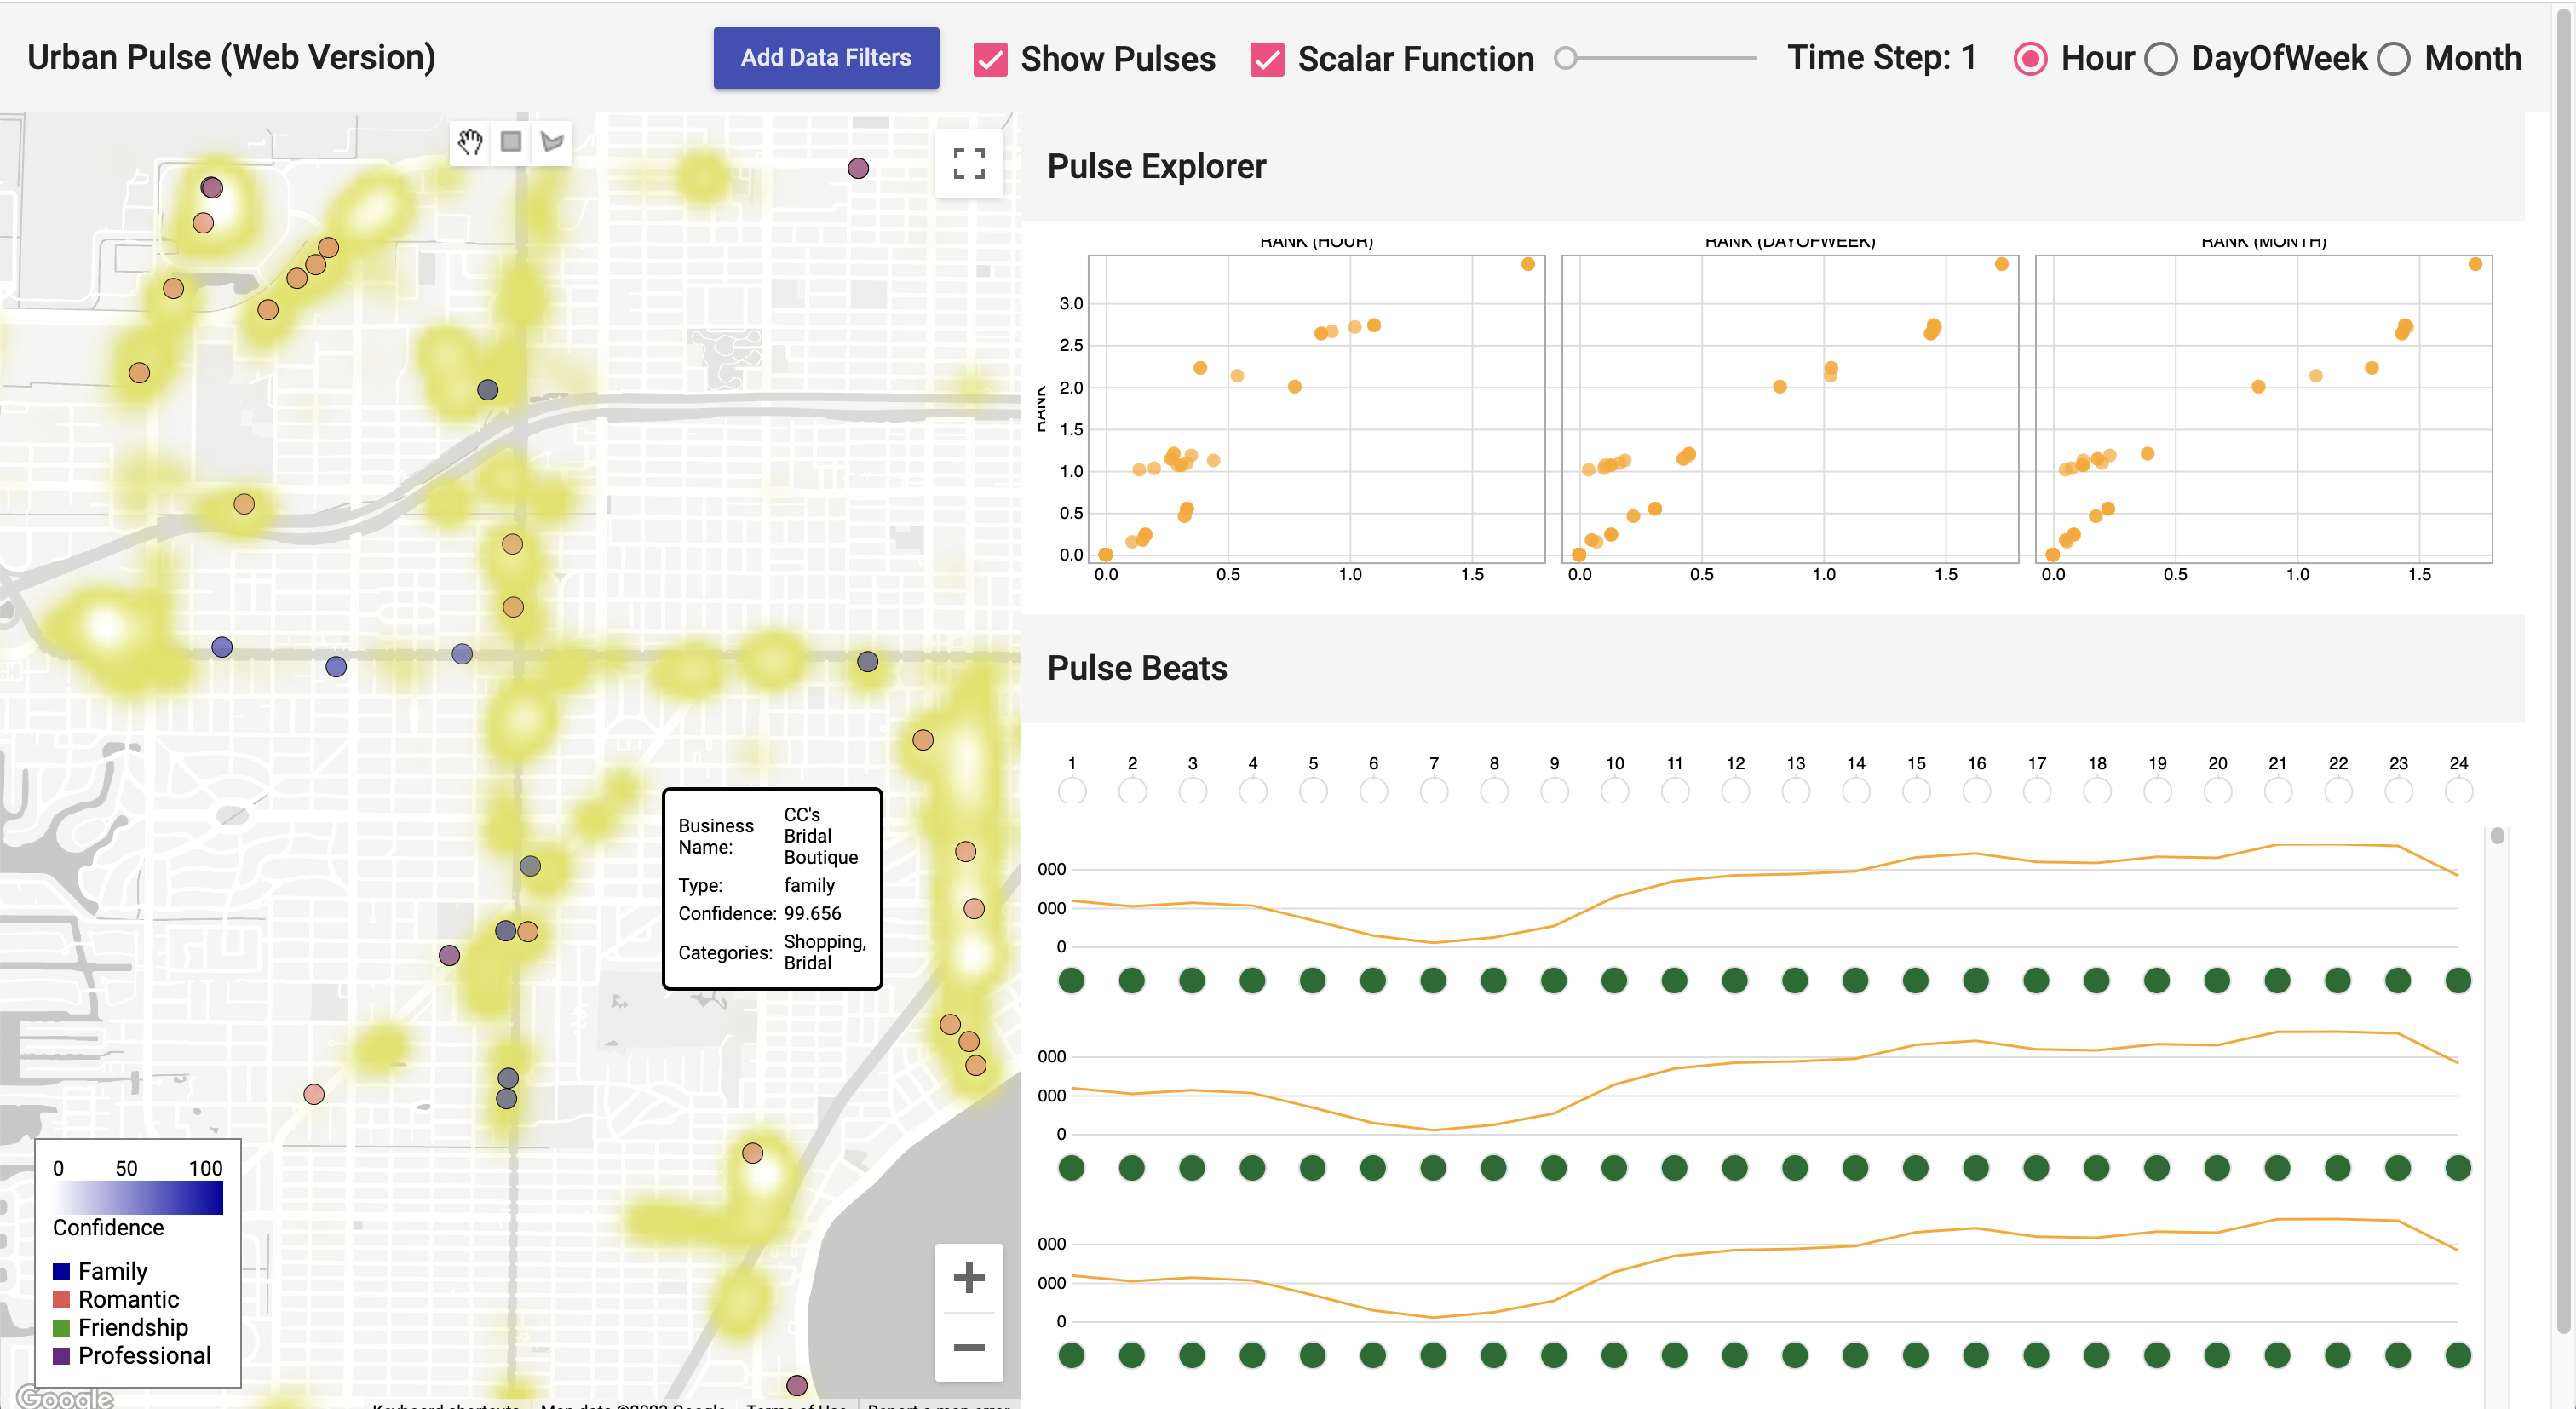
\includegraphics[width=\linewidth,height=8cm]{UrbanPulse}
\caption{Analyzing urban pulses and social fabrics using Yelp dataset for the city of Tampa. The figure demonstrates the spatial distribution of points of interest (POIs) and highlights areas with the highest levels of social interaction. An interactive tool allows users to search for POIs supporting specific types of relationships, providing valuable insights for urban planners and designers.}
\label{fig:teaser}
}

\abstract{
Cities are inherently dynamic, and interesting patterns of behavior often manifest at several key areas of a city over multiple temporal resolutions. Recent technological innovations have enabled the collection of enormous amounts of data that can help in studying these patterns. However, techniques utilizing these data sets typically focus on understanding the data in the context of the city, thus failing to capture the dynamic aspects of the city. In this work, we utilized computational text mining methods\cite{b2} to analyze user reviews from the Yelp Open Dataset in the top five cities with the most points of interest (POIs) to discover how people use these POIs for social interaction. We geolocated the results and spatially analyzed the locations of POIs with reviews mentioning relationship keywords. Additionally, we explored the concept of "urban pulse" which captures the spatio-temporal activity in a city across multiple temporal resolutions \cite{b1}. We used urban pulse to analyze the activity in the top five cities with the most POIs.
Our analysis shows that different parts of the city host different types of relationships, and in some cases, there is little overlap. Certain POIs also support different types of relationships more than others. We also developed an interactive online tool that allows users to select a relationship type of interest (e.g., "family") and search for POIs whose reviews mention these relationships along with their activity across different temporal resolutions.
The findings of this study can be useful for urban planners to reflect upon what kinds of places help support social ties, which ties may need more places for their outings, and how a city can evaluate whether its social infrastructure supply is meeting the demands of residents and visitors.
}

\CCScatlist{
  \CCScatTwelve{Human-centered computing}{Visu\-al\-iza\-tion}{Visu\-al\-iza\-tion techniques}{Treemaps};
  \CCScatTwelve{Human-centered computing}{Visu\-al\-iza\-tion}{Visualization design and evaluation methods}{}
}

\keywords{Urban pulse, computational text mining, points of interest, spatio-temporal activity, social interaction.}
%% Keywords that describe your work. Will show as 'Index Terms' in journal
%% please capitalize first letter and insert punctuation after last keyword
%% \keywords{Radiosity, global illumination, constant time}

%% ACM Computing Classification System (CCS). 
%% See <http://www.acm.org/class/1998/> for details.
%% The ``\CCScat'' command takes four arguments.

%% \CCScatlist{ % not used in journal version
%% \CCScat{K.6.1}{Management of Computing and Information Systems}%
%% {Project and People Management}{Life Cycle};
%% \CCScat{K.7.m}{The Computing Profession}{Miscellaneous}{Ethics}
%% }

%% A teaser figure can be included as follows
%\teaser{
%  \centering
%  \includegraphics[width=\linewidth]{CypressView}
%  \caption{In the Clouds: Vancouver from Cypress Mountain. Note that the teaser may not be wider than the abstract block.}
%  \label{fig:teaser}
%}

%% Uncomment below to disable the manuscript note
\renewcommand{\manuscriptnotetxt}{}

%% Copyright space is enabled by default as required by guidelines.
%% It is disabled by the 'review' option or via the following command:
% \nocopyrightspace


\vgtcinsertpkg

%%%%%%%%%%%%%%%%%%%%%%%%%%%%%%%%%%%%%%%%%%%%%%%%%%%%%%%%%%%%%%%%
%%%%%%%%%%%%%%%%%%%%%% START OF THE PAPER %%%%%%%%%%%%%%%%%%%%%%
%%%%%%%%%%%%%%%%%%%%%%%%%%%%%%%%%%%%%%%%%%%%%%%%%%%%%%%%%%%%%%%%%

\begin{document}

%% The ``\maketitle'' command must be the first command after the
%% ``\begin{document}'' command. It prepares and prints the title block.

%% the only exception to this rule is the \firstsection command
\maketitle


% \begin{IEEEkeywords}
% Urban pulse, computational text mining, points of interest, spatio-temporal activity, social interaction.
% \end{IEEEkeywords}

\section{Introduction}
Urban areas are complex and dynamic environments, constantly changing and evolving over time. As cities grow and change, they present a range of challenges for city planners, architects, and human behavioral experts to understand and navigate. Recent advancements in technology have enabled the collection and analysis of vast amounts of data, providing new opportunities to gain insights into the dynamics of urban environments. 
This paper builds on two previous studies, one focused on the concept of "urban pulses\cite{b1}" and the other on the use of points of interest (POIs) to understand the social fabrics\cite{b2} of urban areas. The concept of urban pulses captures the spatio-temporal activity in a city across multiple temporal resolutions, while POIs provide a rich source of data on how social ties are supported by local amenities. In recent years, with the emergence of online crowdsourcing review sites, such as Yelp, it has become increasingly common for people to share their experiences at POIs and how they interact socially within those POIs. This provides an opportunity to investigate how social interactions occur in urban areas, and how POIs play a role in these interactions. In this paper, we aim to examine the relationship between POIs and social interactions in Indianapolis city.

To achieve our goal, we use computational text mining techniques to analyze user reviews from the Yelp Open Dataset. We extract reviews that mention relationship keywords, such as "friend", "family", "romantic", and "professional" relationships, and classify them into their respective relationship types. We also identify the POIs and POI categories where these relationships are mentioned. In addition, we apply urban pulse analysis to check the activity across multiple temporal resolutions. Our analysis shows that different parts of the city host different types of relationships. For instance, reviews referencing romantic relationships are more likely to occur in downtown areas, while reviews mentioning children are more dispersed in suburban areas. We also find that certain POIs support different types of relationships more than others. For example, restaurants are more likely to be associated with social interactions compared to other POIs. Our study highlights the potential of using online crowdsourcing review sites as a rich source of information about social relationships and their spatial patterns in urban areas. In addition to spatial analysis, we use urban pulses to capture the spatio-temporal activity in the city. We utilized Urban Pulses to analyze and compare different pulses in Indianapolis city. We demonstrate the utility of our approach by exploring the relationship between POIs and social interactions within the city, but we acknowledge that there are limitations to our study, such as the use of only one dataset and the focus on a single city.

The primary contribution of this paper is the integration of urban pulse analysis with POI data to gain a more comprehensive understanding of the social fabrics of urban areas. This approach provides a novel perspective on urban environments that can inform city planning and design decisions. Urban planners can use these findings to reflect upon what kinds of places help support ties, which ties may need more places for their outings, and how a city can evaluate whether its social infrastructure supply is meeting the demands of residents and visitors.

\section{Background}
\subsection{Relationships and Urban Space}

Our study explores the role of POIs in relationship-building, their activity, and social capital, emphasizing the importance of different third places for different communities based on proximity, affordability, and culture\cite{b3}. We draw upon the findings of Mazumdar et al. (2018), who identified POIs, walkability, and land use as the most critical built environmental factors for relationship-building. By analyzing a large, dynamic dataset of online reviews from the Yelp Open Dataset, we show how POIs can provide opportunities for individuals to form new social relationships or revitalize existing ones. Our work also extends classic studies on the built environment's impact on social interaction by responding to theories that certain individuals are excluded from certain destinations due to inaccessibility, exclusivity, or cost. Ultimately, our findings suggest that POIs are a valuable resource for understanding how a city or type of place serves its residents and visitors and can support specific types of social relationships.

\subsection{LBSN and POI Data Analysis}
The field of urban computing has developed numerous methods for gathering and organizing POI data from various sources and contributors\cite{b4}. This research has highlighted the potential for POIs to enhance user experience in recommendation systems, especially in mobile applications. Our analysis utilizes a location-based social network to explore the relationship between place and space through user-generated text content. Prior analyses of LBSN data have used geolocated social media to reveal the emotional state of different areas in a city. POI data from sources such as Twitter, Foursquare, Yelp, and Facebook has been used to examine how culture and weather impact when POIs are open, how their patronage varies over time, and to recommend new POIs to users. The semantics of POI labels have also been used to show how similar POIs cluster geographically and how neighborhoods change over time. Our research builds on this work by disambiguating between different types of social ties (e.g. family, friend) to better understand how people access amenities in different relationships.

\subsection{Urban Pulse}
The concept of urban pulse summarizes the spatio-temporal activity in a city by combining techniques from computational topology with visual analytics to identify, explore and analyze pulses across cities. This is accomplished by modeling the urban data as a collection of time-varying scalar functions over different temporal resolutions, where the scalar function represents the distribution of the corresponding activity over the city. The topology of this collection is then used to identify the locations of prominent pulses in a city, and the pulse is characterized as a set of beats which capture the level of activity at that location over different time steps and resolutions. The urban pulse framework includes a visual interface that can be used to explore pulses within and across multiple cities, and to also compare multiple settings.

\subsection{Scalar functions and Critical Points Determination}
In this project, we focus on modeling data as scalar functions over time, with a particular interest in the spatial region corresponding to a city, represented by a planar domain. The scalar function used is the density function, which captures the level of activity over different locations in a city based on input data points of Yelp Open DataSet. We used the same techniques mentioned in the paper\cite{b1}. The topological features of the scalar function are efficiently computed using a piecewise linear function defined on a triangular mesh, with the function computed for each discrete time step. Critical points of the function are classified based on the behavior of the function within a local neighborhood, and their topological persistence is used to identify locations of interest. The effectiveness of topological persistence as an importance measure has been demonstrated in various applications.
\section{Methods}
\subsection{Data Description}
We used the Yelp Open Dataset, which contains more than 8.6 million reviews for approximately 160,000 businesses\cite{b4} and is publicly available on the web\cite{b5}. The dataset includes posts from October 2004 to January 2021, but we analyzed approximately 2.5 million reviews. For this project, we limited our scope to the top 5 cities with the most POIs count (Table 1). We also reviewed around 5 million checkins and used it to get activity in the city (Section B.)
We found that the median number of reviews per business is 15, and the mean is 42.5. Although 31\% of points of interest (POIs) have fewer than 10 reviews, a few outliers have many reviews. We also observed that around 20\% of businesses had no relationship words in their reviews, and over two-thirds of businesses had fewer than five relationship word occurrences total, which could be due to few total reviews. In later sections, we normalized the relationship word count for each business to get the expected word count per 1,000 reviews, which we called the relationship word rate. To avoid spurious or insignificant results, we only considered POIs with at least 30 reviews and at least 30 relationship-word occurrences.

\begin{table}[htbp]
  \renewcommand{\arraystretch}{1.2}
  \caption{Summary of POI and check-in statistics by city}
  \label{table:poi_stats}
  \centering
  \begin{tabular}{|p{1.3cm}|p{1cm}|p{1cm}|p{1cm}|p{1cm}|p{1cm}|}
    \hline
    \textbf{City} & \textbf{\# POIs} & \textbf{Total Reviews} & \textbf{Median Reviews per POI} & \textbf{Total Check-ins} & \textbf{Median Check-ins per POI} \\
    \hline
    Philadelphia & 14,569 & 813,634 & 17 & 1,838,206 & 17 \\
    \hline
    Tucson & 9,250 & 321,269 & 12 & 772,140 & 13 \\
    \hline
    Tampa & 9,050 & 359,167 & 13 & 918,203 & 16 \\
    \hline
    Indianapolis & 7,540 & 289,986 & 13 & 886,001 & 22 \\
    \hline
    Nashville & 6,971 & 361,162 & 15 & 817,283 & 18 \\
    \hline
  \end{tabular}
\end{table}

We used the Yelp Fusion API Category List\cite{b9} to assign each Point of Interest (POI) to one or more of the 22 top-level categories. However, we considered only businesses within eight categories that were likely to provide a place for social activity, as listed in Table 2. Table 2 is a break down of POIs in top 5 cities mentioned in Table 1. We excluded categories such as "Home Services" (e.g., plumbing, pool cleaners, etc.) that were unlikely to offer social spaces. We note that there is a distinction between "Restaurants" and "Food". "Restaurants" refers to sit-down establishments, while "Food" includes other places where food and drinks are sold, such as coffee shops and food trucks.

\begin{table}[h]
    \centering
    \caption{Number of POIs in each category}
    \small
    \begin{tabular}{|l|r|}
        \hline
        Category & Number of POIs \\
        \hline
        Restaurants & 19133 \\
        Shopping & 9639 \\
        Beauty \& Spas & 6210 \\
        Food & 4942 \\
        Active Life & 3350 \\
        Hotels \& Travel & 2009 \\
        Arts \& Entertainment & 1630 \\
        Nightlife & 1298 \\
        \hline
    \end{tabular}
    \label{tab:businesses}
\end{table}

Relationship keywords were sourced from the American Time Use Survey\cite{b7}, we also used colloquial keywords such as "bae", "boo", and "roommate". Following the methodology of prior work\cite{b2}, the resulting words were grouped into four categories: family, romantic, friendship, and professional (Table 3), according to interpersonal relationship types from sociology and business management sectors. To avoid the need for word stemming during text mining, multiple forms of each relationship word were added to the list (e.g., "friend" and "friends"). The final list of relationship keywords is shown in Table 3, which includes words such as "bff", "partner", "coworker", and "spouse".

\begin{table}[htbp]
    \centering
    \caption{Relationship Keywords}
    \begin{tabular}{|p{1.5cm}|p{6.5cm}|}
    \hline
    \textbf{Type} & \textbf{Words} \\
    \hline
    Family & child(ren), kid(s), daughter(s), son(s), parent(s), mother, mom, father, dad, brother(s), sister(s), siblings, aunt(s), uncle(s), niece(s), nephew(s), cousin(s), grandchild(ren), grandmother, grandma, grandfather, grandpa, grandparents \\
    \hline
    Romantic & partner, relationship, date, boo, bae, sweetheart, fiance, fiancee, girlfriend, gf, boyfriend, bf, spouse, husband, wife \\
    \hline
    Friendship & bff, friend(s), buddy, buddies, pal(s), housemate(s), roommate(s), flatmate(s) \\
    \hline
    Professional & neighbor(s), classmate(s), teacher(s), coworker(s), colleague(s), client(s), boss \\
    \hline
    \end{tabular}
\end{table}

\subsection{Analytical Methods}

\textbf{Scalar function}, that is used in this work, is the
density function. The input data Yelp is provided as a set of
points (data points) having location and time. The density function at
a given location p is defined as the Gaussian weighted sum of data points xi
that are in its neighborhood N(p). Here d() is the Euclidean distance between two points, and $\epsilon$ is the extent of the influence region for a given data point. The neighborhood N(p) is defined
as a circular region centered at p. 

\begin{equation}
f(p) = \sum\limits_{x_i\in N(p)} e^{-\frac{d(p,x_i)^2}{\epsilon^2}}
\end{equation}

In order to efficiently compute the topological features of the scalar function f , it is represented as piecewise linear (PL) function f : K →
R. The planar domain D of the function is represented by a triangular mesh K. The function is defined on the vertices of the mesh and linearly interpolated within each triangle.
To take into account the variation with time, the set of data points
are first grouped together into a discrete set of time steps corresponding to the temporal resolution, and the scalar function is computed for each of these time steps.

\textbf{POI Categorization}: To identify the prevalence of relationship words in Yelp reviews, we employed several preprocessing steps. First, we converted all words to lowercase and replaced punctuation marks with spaces, as reviews often contain possessive forms of words. We then utilized a two-word tokenization approach to identify relationship words preceded by the words "my" or "our" (in cases related to children), as this helped to avoid instances where authors were not referring to their own relationships. Additionally, this approach helped to address the edge cases of POIs with relationship words in their names. We removed any duplicate tokens within individual reviews to capture the overall prevalence of relationship words across reviews, rather than within them. After counting the occurrences of relationship keywords per POI, we calculated the z-scores and p-values to determine the confidence values for each POI. Cdf is cumulative distribution function of the standard normal distribution.

\begin{equation}
\begin{aligned}
\quad z &= \frac{x-\mu}{\sigma}\
\quad p &= 2 * (1 - cdf(z))\
\quad conf &= (1 - p) * 100
\end{aligned}
\end{equation}

This enabled us to more accurately identify businesses with higher or lower-than-expected use of relationship words in their reviews, and gain insights into how people talk about different types of businesses.

\textbf{POI to Pulse Mapping}: In order to map the existing Yelp points of interest (POIs) to urban pulses, it is essential to first determine the critical points using check-in data from the Yelp dataset. Once the critical points (section 2.4) are identified, we proceed to map the POIs using a clustering approach. We map the POIs to the critical point if they are within a user-specified influence region, known as an $\epsilon$-distance, of each other. (Fig 2.) The same $\epsilon$-distance is used for computing the density function in the previous section. After the locations are identified and clustered, they are categorized into three types of beats that capture variations over time\cite{b1}. These beats represent scalar functions that aggregate the data and not the raw data itself. The beats are defined for each possible temporal resolution, thereby enabling a better understanding of how the prominent POIs behave at different times and resolutions.

\begin{figure}
    \centering
    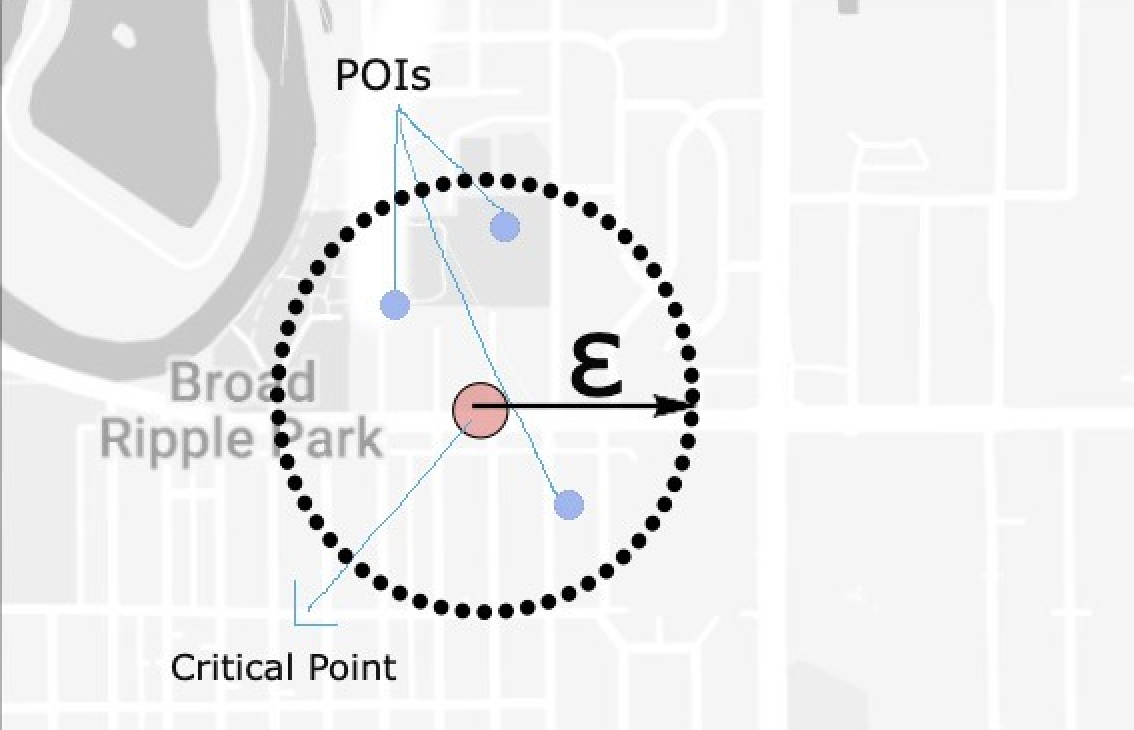
\includegraphics[width=8cm, height=5cm]{Image1.png}
    \caption{Critical Point and POIs within $\epsilon$-distance}
    \label{fig:my_label}
\end{figure}

\section{Results}

\begin{table}[htbp]
  \renewcommand{\arraystretch}{1.2}
  \caption{Occurrence of Relationship Words in Reviews per 1,000}
  \label{table:poi_stats}
  \centering
  \begin{tabular}{|p{1.3cm}|p{1cm}|p{1cm}|p{1cm}|p{1cm}|p{1cm}|}
    \hline
    \textbf{Metro} & \textbf{Words} & \textbf{Family} & \textbf{Rom.} & \textbf{Friends} & \textbf{Profes.} \\
    \hline
    Philadelphia & 167.2 & 94.5 & 17.8 & 41.2 & 13.7 \\
    \hline
    Tucson & 142.3 & 82.1 & 14.6 & 29.8 & 15.8 \\
    \hline
    Tampa & 156.8 & 85.6 & 21.3 & 34.5 & 15.4  \\
    \hline
    Indianapolis & 153.5 & 93.7 & 19.1 & 31.2 & 9.5 \\
    \hline
    Nashville & 169.1 & 100.2 & 15.9 & 40.5 & 12.5 \\
    \hline
  \end{tabular}
\end{table}

Table 4 shows the occurrences of various relationship keywords in the reviews of five cities, namely Philadelphia, Tucson, Tampa, Indianapolis, and Nashville. The most frequent relationship keyword across these cities is "family", with an average of 91.2 occurrences per 1,000 reviews. This is followed by "friends" (average of 17.7 per 1,000 reviews), "romantic" (average of 17.7 per 1,000 reviews), "professional" (average of 11 per 1,000 reviews). It is interesting to note that the occurrences of these relationship keywords vary across the cities, with Nashville having the highest average occurrences of relationship keywords (169.1 per 1,000 reviews) and Tucson having the lowest (142.3 per 1,000 reviews). These differences may reflect the cultural, social, and economic characteristics of these cities.

Spatial analysis is a powerful tool that allows us to investigate how the physical environment influences human behavior and social interactions. By examining the spatial distribution of certain social ties in different cities and neighborhoods, we can gain valuable insights into the factors that promote or hinder the formation of these ties. For example, research has shown that urban areas with high levels of walkability and public transit use tend to promote social ties by creating more opportunities for face-to-face interaction\cite{b8} and reducing reliance on private vehicles. Similarly, neighborhoods with strong community organizations and social networks may provide a supportive environment for the formation of close-knit relationships such as friendships and family ties. Further research is needed to explore the complex relationship between spatial patterns and social ties, and to identify ways to promote more equitable and supportive social environments. By leveraging the power of spatial analysis, we can gain a deeper understanding of the social dynamics of our cities and communities, and work towards building more inclusive and connected societies.
\section{Interactive Tool}

\subsection{Overview}

This interactive tool is an extension of the Urban Pulse interactive tool\cite{b1} and all the interaction strategies and widgets are of similar functionality. The interactive tool (Fig. 1) developed in this research combines the Map View and the Pulse Monitor components to allow users to explore the city's POIs by both POI type and the type of relationships they support. The tool is designed to enable users to gain a broad overview of the city's POIs, zoom and filter to seek finer details on individual entities and analyze the different properties of the pulses along with the activity across different temporal resolutions. The purpose of the tool is to support the exploration of pulses by both POI type and the type of relationships they support, in one or more cities and to enable the comparison of pulses across different scenarios within a city. The tool is intended for use by locals and tourists looking to find a venue to patronize under certain social contexts, as well as professionals aiming to understand how city layouts support different social relationships or where to put new businesses. The interactive tool (Fig. 3) is a powerful and innovative way to explore and analyze the relationship between POIs and social relationships in cities, providing users with a unique and informative experience.

\subsection{Features}
The interactive tool in Fig 1 shows the interface of the interactive tool. They can then select the relationship types (Fig. 4) they are interested in (e.g., "professional" or "romantic") using checkboxes, and optionally filter by POI type (e.g., "Restaurants" or "Arts \& Entertainment") using a dropdown menu. The tool offers several options to display the data: the raw number of relationship words, relationship word rate (number of words per 1000 reviews), or the percentage of relationship keywords in their reviews under that type. Users can limit the number of POIs to display on the map, where POIs with the highest relationship word rate (or raw count, or percent of words under the selected type) are shown.

Each point in the map is also color-coded based on the level of confidence in the presence of the selected relationship type in the reviews. POIs are symbolized by one of four different colors according to relationship type, and the color intensity increases with the level of confidence. Darker shades of a color indicate a higher confidence percentage of that relationship type in the reviews of that POI. The tool allows users to hover over POI points to see tooltips that include the name of the business and details about the relationship word occurrences in its reviews. Furthermore, users can limit the number of POIs to show on the map, wherein POIs with the highest relationship word rate (or raw count, or percent of words under the selected type) are drawn first. The tool also includes a sortable table of the POIs that are currently in view, which includes additional attributes such as the total number of reviews. Users can select a POI in the table and "jump" to it on the map, enabling exploration of different neighborhoods and serving as a reference through search capabilities. By providing zoomed-out snapshots of cities’ POIs, it also allows users to visually distinguish the prevalent relationships supported by various parts of a city and thus evaluate different parts of the city with relationships in mind. The tool also includes a sortable table of the POIs currently in view, which includes additional attributes such as the total number of reviews. Users can select a POI in the table and "jump" to it on the map. This feature enables the exploration of different neighborhoods and serves as a reference through search capabilities to look up specific POIs.

\begin{figure}
    \centering
    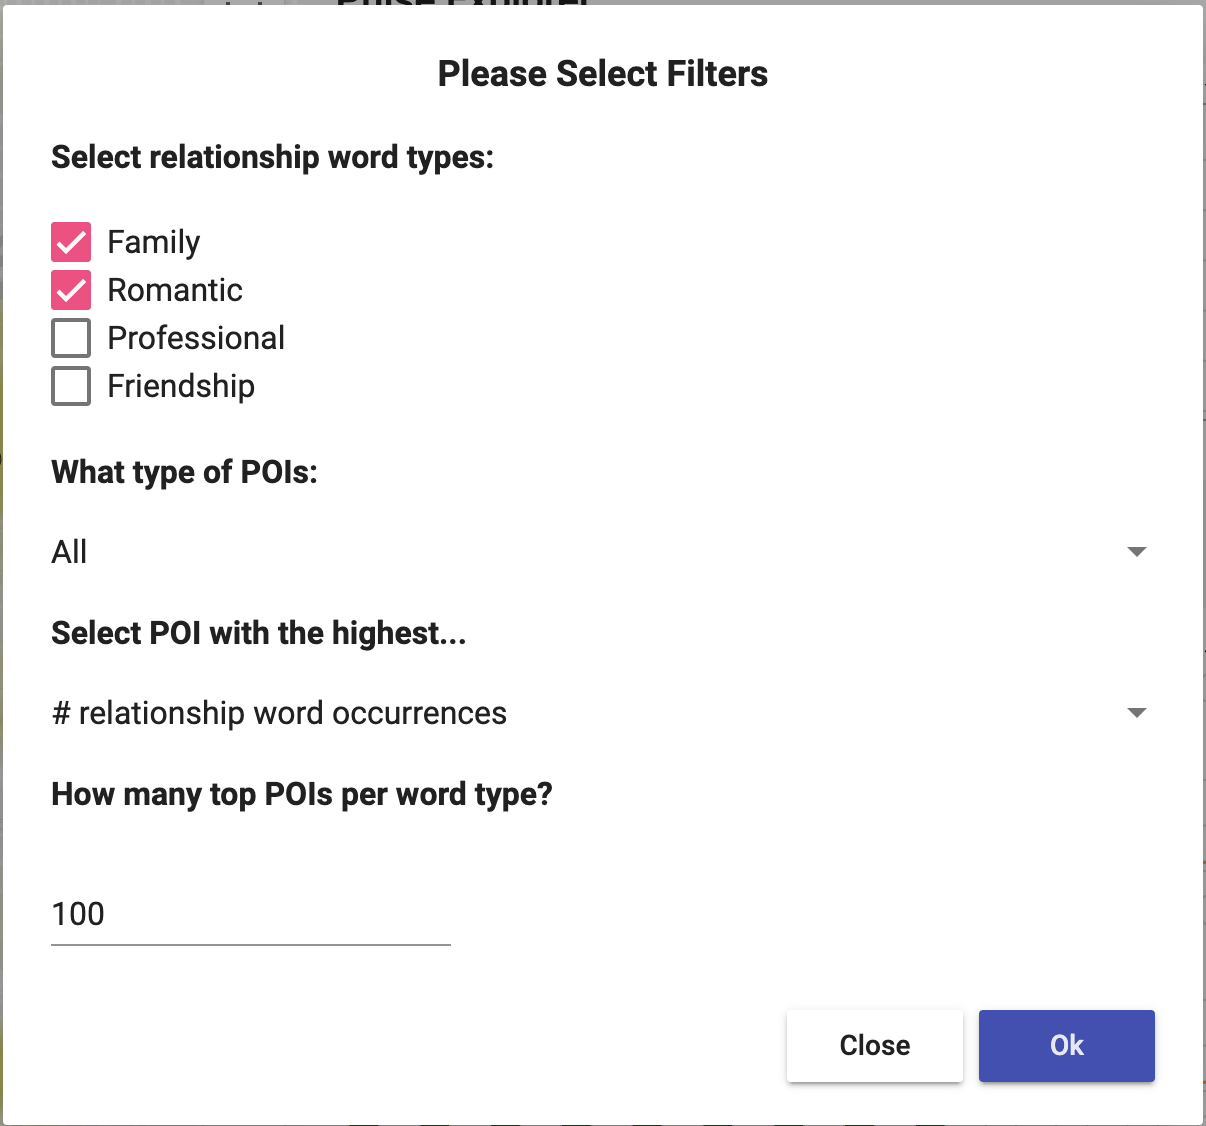
\includegraphics[width=\linewidth, height=6cm]{Filters.png}
    \caption{Options to interact with and filter on the tool}
    \label{fig:my_label}
\end{figure}


\section{Limiations and Future Work}

Despite the insights provided by our study, there are several limitations that must be acknowledged. First, our reliance on user-generated content may result in inaccurate reflections of actual social ties and relationships. Additionally, the keywords we used may not have been sufficient to capture the wide variety of relationships that use POIs. Our analysis was also limited to English-oriented keywords, which may have missed out on relationship words that are not in English, such as abuela for "grandmother" in Spanish. Furthermore, the term "partner" is ambiguous as it could refer to a professional or romantic relationship, which could lead to misinterpretation of results. Lastly, our analysis only included a limited number of cities, which may not be representative of other regions.

Further research and analysis could be conducted to explore the spatio-temporal activity and social ties of a region, which could provide valuable insights. Future studies should also explore more nuanced and inclusive approaches to dealing with relationship words. They should also consider using keywords in other languages to ensure more comprehensive analyses. Additionally, studies could explore the use of location-based social networks to suggest POIs based on who the user wants to spend time with. Disaggregating restaurant/food categories into subtypes may also be helpful in identifying stronger connections between relationship types and locales. Finally, future work could focus on addressing the issue of reinforcing or "branding" particular spaces as suitable or unsuitable for certain activities. In terms of technical limitations, the spatial analysis may not have considered the density of POIs that do not have relationship keywords. Further work is needed to disaggregate the restaurant/food categories into subtypes, such as upscale dining, sports bars, hot pot restaurants, etc. which may be used by pairs and groups for different purposes. Lastly, users should be cautioned that these results only present one perspective of cities and social network relationships, and a lack of POIs or information about a place does not imply that a place is not suitable for social life or activities (and vice versa).

\vspace{12pt}


\begin{thebibliography}{00}
\bibitem{b1} Miranda, F., Doraiswamy, H., Lage, M., Zhao, K., Gonçalves, B., Wilson, L., Hsieh, M., \& Silva, C. T. (2016). Urban Pulse: Capturing the Rhythm of Cities. ArXiv. https://doi.org/10.1109/TVCG.2016.2598585
\bibitem{b2} Bendeck, Alexander, and Clio Andris. "Text Mining and Spatial Analysis of Yelp Data to Support Socially Vibrant Cities." (2022).
\bibitem{b3} Sharon Zukin. 1998. Urban lifestyles: diversity and standardisation in spaces of
consumption. Urban Studies 35, 5/6 (1998), 825–839.
\bibitem{b4} Jennings Anderson, Dipto Sarkar, and Leysia Palen. 2019. Corporate editors
in the evolving landscape of OpenStreetMap. ISPRS International Journal of
Geo-Information 8, 5 (2019), 232.
\bibitem{b5}Yelp, Inc. 2022. Fast Facts. https://www.yelp-press.com/company/fast-facts/
default.aspx
\bibitem{b6} Yelp, Inc. 2022. Yelp Open Dataset: An All-Purpose Dataset for Learning. https:
//www.yelp.com/dataset
\bibitem{b7} U.S. Bureau of Labor Statistics. 2020. American Time Use Survey (ATUS). https:
//www.bls.gov/tus/database.html
\bibitem{b8} Kim, S., \& Kim, S. (2018). Social capital and urban public transportation use: Evidence from the United States. Journal of Transport Geography, 71, 142-150.
\bibitem{b9} Yelp, Inc. 2022. All Category List - Yelp Fusion. https://www.yelp.com/developers/
documentation/v3/all\_category\_list
\end{thebibliography}

%\bibliographystyle{abbrv}
\bibliographystyle{abbrv-doi}
%\bibliographystyle{abbrv-doi-narrow}
%\bibliographystyle{abbrv-doi-hyperref}
%\bibliographystyle{abbrv-doi-hyperref-narrow}

\bibliography{proposal}
\end{document}

